%===========================================================
%                              Choix de track
%===========================================================
% Une des trois options 'parallelisme', 'architecture', 'systeme' 
% doit être utilisée avec le style compas2016
\documentclass[parallelisme]{compas2016}

\usepackage[utf8]{inputenc}
\usepackage[T1]{fontenc}

\usepackage{url}
\usepackage{graphicx}
\usepackage{caption}
\usepackage{subcaption}
\usepackage{subfig}
\usepackage{wrapfig}
\usepackage{multirow}
\usepackage{boxedminipage}
\usepackage{xspace}
\usepackage{listings}
\usepackage{listingsutf8}
\usepackage{verbatim}
\usepackage{parcolumns}
\usepackage{color}
\usepackage[usenames,dvipsnames,svgnames,table]{xcolor}
%Prevents floating item to "jump" between sections
\usepackage[section]{placeins}
\usepackage{booktabs}
\usepackage{tkz-graph}
\usepackage{setspace}




\renewcommand{\ttdefault}{pcr}
\lstset{
	tabsize=4,
%	frame=single,
	breaklines=true,
	basicstyle=\ttfamily,
	frame=tb,
	framerule=0.2pt,
%	frameround={tttt},
	showstringspaces=false,
	language=c,
%	linewidth=0.95\textwidth,
	keywordstyle=\color{black}\bfseries,
%	keywordstyle=\color{blue},
	commentstyle=\color{OliveGreen},
	stringstyle=\color{red}\itshape,
	inputencoding=utf8/latin1,
	numbers=left,
	numberstyle=\tiny,
	numbersep=5pt,
% OMP define
emph={\#,pragma, taskwait, omp, task, depend}, emphstyle=\color{RoyalBlue}\bfseries,
emph={[2]in,inout,out,cw}, emphstyle={[2]\color{BrickRed}\bfseries},
emph={[3]tied,untied,shared}, emphstyle={[3]\color{Gray}\bfseries},
emph={[4]lu0,fwd,bdiv,bmod}, emphstyle={[4]\color{DarkGreen}\bfseries},
emph={[5]cw}, emphstyle={[5]\color{DarkViolet}\bfseries},
    %moredelim=**[is][\only<3>{\color{red}}]{@}{@},
}
\lstdefinestyle{smaller}{basicstyle=\scriptsize\ttfamily}
\lstMakeShortInline|
%===========================================================
%                               Title
%===========================================================

\toappear{1} % Conserver cette ligne pour la version finale

\begin{document}

\title{Amélioration des stratégies d'ordonnancement sur architectures NUMA à l'aide
des dépendances de données}

\author{Philippe Virouleau}
\address{Inria,\\
   Univ. Grenoble Alpes,  CNRS, Grenoble Institute of Technology, LIG, Grenoble, France\\
   philippe.virouleau@inria.fr\\
}
\date{}


\maketitle

\newcommand{\benchs}{KASTORS }
\newcommand{\kaapi}{\textsc{\mbox{Xkaapi}}\xspace}
%===========================================================         %
%R\'esum\'e
%===========================================================  
\begin{abstract}
Le récent ajout des dépendances de données à la norme OpenMP 4.0 offre
au programmeur une manière flexible de synchroniser les tâches.
Grâce à cela, le compilateur et le support exécutif peuvent tous les deux savoir
exactement quelles données sont lues ou écrites par quelles tâches, et comment
ces données peuvent éventuellement être réutilisées au cours de l'exécution du
programme.
Les performances sur architectures NUMA peuvent être fortement impactées par
le placement des données et l'ordonnancement des tâches. Les informations présentes
dans les dépendances de données peuvent être utilisées pour contrôler le placement physique des données,
ainsi que pour contrôler les stratégies de placement des tâches en
fonction de la topologie.
Ce papier présente plusieurs heuristiques pour ces stratégies, et leurs implémentations
dans notre support exécutif OpenMP : \kaapi.
Nous présentons également nos évaluations sur des applications d'algèbre linéaire,
exécutées sur une machine NUMA à 192 cœurs, et comparées aux stratégies proposées
par l'état de l'art.
  \MotsCles{OpenMP, tâche avec dépendances, support exécutif, NUMA, ordonnancement}
\end{abstract}

	
\section{Introduction}

Bien que les architectures à temps d'accès mémoire non uniforme (NUMA) soient
aujourd'hui l'un des choix les plus populaire pour créer des grosses machines à mémoire
partagées, il est toujours compliqué de pouvoir les exploiter à leur plein potentiel.
Compte tenu de la différence de temps d'accès en fonction de la distribution physique
de la mémoire (une donnée proche sera accédée beaucoup plus rapidement qu'une donnée distante),
contrôler le placement des données tout au long de l'exécution d'une application
est donc l'un des points clés pour améliorer sa scalabilité et ses performances.

Les environnements de programmation parallèle tels que OpenMP sont devenus très
populaires pour exploiter les machines à mémoire partagée avec plusieurs centaines de cœurs.
Ils offrent un moyen d'exprimer beaucoup de parallélisme à grain fin, tout en
ayant un coût relativement faible. La plupart d'entre eux fournissent également
un moyen d'équilibrer dynamiquement la charge de travail sur tous les processeurs,
mais les plus standard ne fournissent pas de moyen explicite de gérer la localité
des données sur des systèmes NUMA.

L'ajout récent des dépendances de données au modèle de programmation par tâches
d'OpenMP fourni au support exécutif des informations précises, notamment concernant
quelle partie de l'application utilise quelle donnée.
L'ordonnanceur de tâches peut donc se baser sur ces informations pour affecter
les tâches aux processeurs, et implémenter des stratégies dédiées aux architectures
NUMA, comme montré dans ce papier.

Ce papier décrit plusieurs stratégies que nous avons implémenté dans notre support
exécutif \kaapi. Nous avons identifié trois points majeurs dans l'ordonnanceur qui
peuvent impacter les applications parallèles pour systèmes NUMA : la distribution
de données, l'assignation des tâches prête, et la manière de parcourir l'architecture
pour effectuer l'équilibrage de charge.

Ce papier les décrit et les évalue, en montrant leur impact sur les performances
d'applications s'exécutant sur une machine NUMA à 192 cœurs.
Nous les comparons également aux stratégies de l'état de l'art implémentées dans \kaapi.

Le plan de ce papier est le suivant : dans la partie~\ref{sec:background},
nous donnons quelques informations essentielles sur les architectures NUMA et
le modèle de tâches avec dépendances. Ensuite dans la partie~\ref{sec:contributions}
nous décrivons les idées, stratégies, et détails d'implémentation que nous avons
utilisé pour améliorer les performances du système exécutif. La partie~\ref{sec:performances-evaluation}
présente les évaluations de performances. Enfin nous présentons des travaux de l'état
de l'art dans la partie~\ref{sec:related-work}, avant de conclure.


\section{Description des systèmes NUMA et de leur exploitation}

\label{sec:background}
\subsection{Hardware background}
\label{sec:hardware}
La plupart des architectures à mémoire partagée actuelles sont basées sur le modèle NUMA,
dans lequel la mémoire est physiquement répartie sur plusieurs nœuds attachés
aux processeurs. La plupart des vendeurs relient ces nœuds suivant une logique
hiérarchique, ce qui permet de construire des machines à plusieurs centaines de cœurs.

Le temps d'accès à de la mémoire située sur un nœud local est plus rapide que celui
pour accéder à de la mémoire située sur un nœud distant, il est donc important
de le prendre en compte lors de l'exécution du programme.

Nous avons effectué nos expériences sur une machine SGI UV2000, constituée de
24 nœuds NUMA, possédant chacun un processeur Intel Xeon E5-4640 à 8 cœurs,
le tout formant un total de 192 cœurs. Nous utilisons le nom Intel192 pour faire
référence à cette machine dans le papier.

\subsection{Software background}

Afin d'exploiter les grosses architectures à mémoire partagée, le programmeur a besoin :
\begin{enumerate}
    \item d'exprimer beaucoup de parallélisme à grain fin, pour profiter au maximum du nombre
      important de processeurs disponibles;
    \item de contrôler l'exécution de l'application, en particulier la manière dont sont distribuées
      les données.
\end{enumerate}

Les environnements de programmation parallèle à base de tâches fournissent un moyen
d'exprimer le parallélisme à grain fin. OpenMP~\cite{openmp40}, le standard utilisé
en pratique pour la programmation des architectures à mémoire partagée, supporte
le parallélisme à base de tâches avec dépendances de données depuis la version 4.0.

\subsubsection{Un aperçu du modèle de tâches d'OpenMP}

Une \emph{tâche} OpenMP peut être vue comme une \emph{unité indépendante de travail} qu'un thread
OpenMP peut exécuter. Les tâches peuvent être exécutées par un thread quelconque
de la région parallèle.
Gérer les tâches pendant l'exécution est bien moins coûteux que de créer et synchroniser
des threads, le programmeur peut donc considérer que certaines parties de son code
trop petites pour être parallélisées avec des threads peuvent l'être avec des tâches.

Dans la norme OpenMP 3.0, la synchronisation des tâches est effectuée à l'aide du
mot clé |taskwait|, imposant l'attente de la complétion de toutes les tâches
de la région parallèle courante.

La norme 4.0 enrichie ce concept en introduisant le mot clé |depend|, qui permet
de spécifier le mode d'accès des variables utilisées par une tâches pendant son exécution.
Le mode d'accès peut être soit |in|, |out|, ou |inout|, en fonction de si la
variable correspondante est respectivement lu par la tâche, écrite, ou bien les deux.
Cette information peut être analysée par le support exécutif, qui décidera si
la tâche est prête à être exécutée ou si elle doit attendre la complétion d'une
autre tâche.


%\subsubsection{Un exemple de la suite de benchmarks KASTORS}
%La figure~\ref{lulst} montre l'implémentation d'une factorisation de Cholesky
%à l'aide des tâches avec dépendances d'OpenMP.
%Cet algorithme est très proche de celui implémenté dans la suite de benchmark
%KASTORS~\cite{virouleau:hal-01081974}, utilisée dans nos expérimentations.

%Dans certaines situations, la programmation par tâches avec dépendances permet
%plusieurs scénarios d'exécution valide de l'application, ce qui permet au
%support exécutif plus de liberté dans l'ordonnancement des tâches.
%Dans l'exemple, il y a plusieurs instances des BLAS |dtrsm|, |dsyrk|, et |dgemm|
%qui peuvent s'exécuter de manière concurrente.

%\begin{figure}[tbp]
%\hrule
%\begin{minipage}[t]{.43\textwidth}
%\begin{lstlisting}[frame=none,style=smaller,showlines=true,label=lst:LU-deps]{lst:LU-deps1}
%for (size_t k=0; k < NB; ++k) {
%#pragma omp task shared(A) \
  %depend(inout: A[k][k])
  %dpotrf(NB,&A[k][k]);

  %for (int m=k; m < NB; ++m) 
%#pragma omp task shared(A)\
  %depend(in: A[k][k]) \
  %depend(inout: A[m][k])
    %dtrsm(NB,&A[k][k],&A[m][k]);

%\end{lstlisting}
%\end{minipage}\hfill
%\begin{minipage}[t]{.485\textwidth}
%\begin{lstlisting}[frame=none,style=smaller,label=lst:LU-deps,firstnumber=12]{lst:LU-deps2}
  %for (int m=k; m < NB; ++m) {
%#pragma omp task shared(A)\
  %depend(in: A[m][k]) \
  %depend(inout: A[m][m])
   %dsyrk(NB,&A[m][k], &A[m][m]);

    %for (int n=k; n < m; ++n)
%#pragma omp task shared(A)\
  %depend(in: A[m][k],A[n][k])\
  %depend(inout: A[m][n])
     %dgemm(NB,
       %&A[m][k],&A[n][k],&A[m][n]);
  %}
 %}
%\end{lstlisting}
%\end{minipage}
%\hrule
%\caption{Cholesky factorization with OpenMP-4.0 task dependencies} \label{lulst}
%\end{figure}


\subsubsection{The way we execute task-based applications}

Most task-based programming environments rely on a work-stealing execution model, originally introduced in Cilk~\cite{cilk5}. 
Work-stealing is indeed often considered when it comes to dynamically balance the workload among processing units. 
The work-stealing principle can be summarized as follows. 
An idle thread, called a thief, initiates a steal request to a randomly selected victim. 
On reply, the thief receives a copy of one ready task, leaving the original task marked as stolen.
Coherency between a thief and its victim is ensured by a variant of Cilk's T.H.E protocol, also described in \cite{cilk5}.

The runtime system we develop, called \kaapi, also implements the work-stealing execution model to execute OpenMP task-based applications.
The runtime creates a system thread, called a \emph{kproc}, for each processing unit to be used.
On a NUMA multicore machine, a processing unit is a core.
A kproc creates tasks and pushes them on its own work queue, which is implemented as a stack.
The enqueue operation is very fast : it takes around ten cycles on modern x86/64 processors~\cite{libkomp}.
As in Cilk, a  running \kaapi task can create children tasks. 
%During the execution of a task-based application, if a kproc encounters a task that is marked as stolen, it suspends its execution and switches to
%the work stealing scheduler that waits for dependencies to be met before
%resuming the kproc execution. 
Depending on the number of tasks per thread, \kaapi implements two strategies to find a ready task.
If the number of tasks is lower than a threshold, \kaapi follows the Cilk's~\textit{work first principle}. 
In that case, the thief iterates through the victim's stack queue from 
the least recently pushed task to the most recently one and it computes true
data-flow dependencies for each task until a ready task is found. If the number of tasks is greater than the threshold, 
the data flow graph is built and the thief picks a task from the victim's list of ready tasks~\cite{Bleuse2014}.
By the nature of our benchmarks, this latter strategy is de facto selected and we developed new NUMA aware strategies.



\section{Using OpenMP tasks dependencies to improve tasks and data
  placement on NUMA machines}
\label{sec:contributions}

In this section, we describe how the runtime system can have a positive impact on the application execution using the information provided by data dependencies.
The following sections describe the way we adapted the behavior of the runtime system to control data placement during the initialization phase, when data will be allocated and accessed for the first time, and how we modified the way tasks that perform the actual computations are dynamically assigned to processors while maximizing data locality.

\vspace*{-1ex}
\subsection{Inside the \kaapi task-based runtime system}

This section describes some of the key internal structures and mechanisms of the \kaapi runtime system.

\vspace*{-1ex}
\subsubsection{The way \kaapi models the architecture.}


\kaapi sees the architecture topology as a hierarchy of \verb/places/.
A \verb/place/ is a list of tasks associated with a subset of the machine processing units.
\kaapi's places are very similar to the notion of \emph{shepherd} introduced in \cite{DBLP:journals/ijhpca/OlivierPWSP12}, or ForestGOMP's \emph{runqueues}~\cite{BroFurGogWacNam10IJPP}.
\kaapi most of the time only considers two levels of places : node-level places, which are bound to the set of processors contained in a NUMA node, and processor-level places, which are bound to a single processor of the platform.
This way, at the processor level one \verb/place/ is associated to each of the physical cores, and
at the NUMA node level one \verb/place/ is associated to each of the NUMA nodes.


\subsubsection{The way \kaapi enables ready tasks and steals them.}
The scheduling framework in \kaapi~\cite{Bleuse2014} relies on virtual functions for \textit{selecting a victim}, \textit{selecting a place} to push a ready task and \textit{pushing} a set of initial ready tasks.
When a processor becomes idle, the runtime system calls a function, called  \verb/WSselect/ for \emph{work-stealing select}, to browse the topology to find a place from which stealing a task from the place task queue.

The completion of a task may unlock the execution of some of its children in the dependency graph.
This means marking them as ready for execution and pushing at least one of them to a place.
Once again, there are many ways of selecting the place where to push ready tasks, implemented in strategies we refer to as \verb/WSpush/, for \emph{work-stealing push}.
Before parallel computation begins, the runtime system distributed the set of ready tasks accordingly to the strategy defined by \verb/WSpush_init/.

These functions are the three main entry points to specify a scheduling algorithm in \kaapi. 

\subsection{Controlling data distribution on a NUMA system}

Controlling the way data are allocated on a NUMA system requires a good understanding of the underlying memory architecture.
Application programmers can achieve this using dedicated tools or libraries, like libNUMA's \verb!numactl!~\cite{DBLP:journals/corr/abs-1101-0093}, which can be used to set a default memory allocation policy for the whole application.
For example, the \verb!--interleave=all! memory policy spreads out all the memory pages of dynamically allocated variables, over all the NUMA nodes of the machine.
This policy is widely used on NUMA systems in conjunction with dynamic parallelism, like task-based programs, as it distributes the memory traffic over all the memory controllers, making processors "\emph{all equally bad}" when it comes to memory access.
To better control data placement, parallel application programmers are used to relying on the \emph{first-touch} allocation policy, which is the default behavior for memory allocation on most Linux systems.
This allows allocating memory pages when they are accessed for the first time.

To better control data distribution on NUMA systems, we propose two different approaches :
\begin{itemize}
\item either the application programmer explicitly allocates data on specific NUMA nodes of the machine through a dedicated API we provide~\cite{Durand2013} (\verb!omp_locality_domain_allocate_XXX!) where \verb/XXX/ may be a bloc cyclic data distribution for one or two-dimensional arrays over MAMI~\cite{BroFurGogWacNam10IJPP};
\item or the application programmer only marks some regions of code that initialize data to give the runtime system the opportunity to map the corresponding tasks to make the first-touch allocation policy indirectly apply the data distribution we target. Indeed, Olivier et al.~\cite{Olivier:2012:CMW:2388996.2389085}
have shown that specifying affinity for initialization tasks can lead to huge improvement over locality oblivious techniques.
To avoid remote memory accesses, the threads must access the data during the computation phase the exact same way it was accessed during the initialization phase, which is very difficult to guarantee with dynamic task-based parallelism.
We extend the OpenMP runtime in two ways. First, by adding functions to provide a dedicated API: \verb!omp_set_affinity! to  make the runtime map the next task to a specific NUMA node. Secondly, by extending scheduling heuristics to take into account task's dependencies to better map ready tasks.
\end{itemize}
Both of these approaches give the runtime system a way of keeping track of where the memory pages associated with the application data are actually stored.
This information is then used to guide the way we perform task creation and load balancing.

\subsection{Distribution of initial ready tasks : WSpush\_init strategies}
We refer to \emph{initial tasks} when considering the sources of a task dependency graph, usually declared at the beginning of an OpenMP parallel region.
These tasks are basically the first ones to be marked as ready and to be distributed over the platforms' places.
We have implemented two initial tasks distribution strategies : \verb!cyclicnuma! which distributes the tasks in a round-robin fashion over the NUMA nodes, and \verb!randnuma! which randomly distributes the tasks over the NUMA nodes.
Note that unlike \verb!numactl!, the strategies we implemented consider the whole data appearing in the OpenMP task \verb!depend! clause instead of working at the page level. In other words, while the two memory pages holding an 8K-wide array would be distributed on different nodes by \verb!numactl --interleave=all!, they are always assigned to the same NUMA node when using one of our data distribution strategies.

\subsection{Distribution of ready tasks : WSpush strategies}

This section describes four different ways of pushing ready tasks to a NUMA system places.
Two of them are data-oblivious while the other two rely on the dependencies expressed using the \verb!depend! keyword on OpenMP tasks.

The \verb/pLoc/ strategy makes a processor push ready tasks to
    its own place, while the \verb/pLocNum/ strategy makes a processor push ready tasks to the place of its NUMA node (\emph{local NUMA node}).
The \verb/pNumaW/ strategy pushes tasks on the node-level place corresponding to the NUMA node where most of their output data are allocated to (W stands for Write).
The last WSpush strategy, called \verb/pNumaWLoc/, behaves almost the same than \verb!pNumaW! except that if
    the data are allocated to the NUMA node of the processor pushing the task, we directly push the task to this processor's place instead of pushing it to the node-level place (Loc stands for Local).
    
    It's important to note that \verb!pLoc! and \verb!pLocNum! does not take initial data placement into account, while \verb!pNumaW! and \verb!pNumaWLoc! are both aware of where a task's data are physically allocated and which of them are written, thanks to the OpenMP \verb!depend! keyword.

\subsection{Dynamic load balancing using work-stealing : WSselect strategies}

Another important step when implementing work-stealing is the selection of the victim processor we want to steal from.
This section describes the selection strategies we implemented, that take the architecture memory hierarchy into account.
The first two strategies, \verb!sRand! and \verb!sRandNuma! are similar to those studied in~\cite{DBLP:journals/ijhpca/OlivierPWSP12}
and distinguish two levels of hierarchy : the processor level and the NUMA node level.
\verb/sRand/ selects a random processor's place while \verb/sRandNuma/ selects a random NUMA node's place.
We additionally implemented several strategies mixing both levels of hierarchy,
described below.

\begin{itemize}
  \item \verb/sProcNuma/ : First, we browse the processor's place. Upon failure, we browse the topology in the following order : we first browse one of the neighbor processors ; when all the neighbors have been visited, we browse the local NUMA place ; we continue by browsing all the processors' places from a random remote node and we eventually consider the place of its NUMA node.
  \item \verb/sNumaProc/ : This strategy is similar, except we always look at the
    NUMA place before looking at the processors' place.
  \item \verb/sProc/ : In this strategy the stealer will visit only the
    processors' places and its own NUMA place.
  \item \verb/sNuma/ : In this strategy the stealer will visit only NUMA places
    and its neighbors. 
\end{itemize}

Like proposed in \cite{Olivier:2012:CMW:2388996.2389085}, all these strategies come in two versions : a \verb!strict! version in which we prevent processors from stealing from other NUMA nodes to improve data locality and a \verb!loose! version where these restrictions do not apply.


\section{Evaluation}
\label{sec:performances-evaluation}

We ran all our experiments on the Intel192 machine described in section \ref{sec:hardware}.
We evaluated our strategies using the KASTORS~\cite{virouleau:hal-01081974}\footnote{git available at https://scm.gforge.inria.fr/anonscm/git/kastors/kastors.git, tag "tag-europar16"} benchmark suite.
More specifically, we used the dependent tasks version of the blocked QR factorization
(\verb/dgeqrf_taskdep/), and of the blocked Cholesky factorization (\verb/dpotrf_taskdep/).
These applications rely on kernels from BLAS and LAPACK libraries provided by OpenBLAS 2.15.
We used the OpenMP GCC compliant runtime libKOMP~\cite{libkomp} based on \kaapi runtime system. We tagged the version we used on \kaapi's
git repository\footnote{https://scm.gforge.inria.fr/anonscm/git/kaapi/kaapi.git } in the branch \emph{public/europar2016}.
For all of the above applications, we used the GCC 5.2.0 compiler.
We also made our execution log files public\footnote{https://github.com/viroulep/europar-2016-public}, as well as all the scripts we used, so that
anyone may reproduce our data analysis.

\subsection{Impact of the data distribution}

We first evaluated the impact the initial data distribution has on the application performance. We did an evaluation for multiple matrix sizes and block sizes,
as well as multiple combinations of WSpush and WSselect strategies. Figure \ref{fig:eval-distrib} reports the
results we obtained for the Cholesky application, on 32K-wide matrices divided into blocks of 512$\times$512 elements. We observed similar behavior running Cholesky on different matrix sizes (16K to 64K) and block sizes (256 to 1024).
The lower double dashed horizontal line is the GCC performance baseline using
sequential initialization. The middle dashed line is the same experiment using
\verb/numactl/. The upper solid line is the GCC baseline using parallel initialization.

\begin{figure}[t]
  \centering
  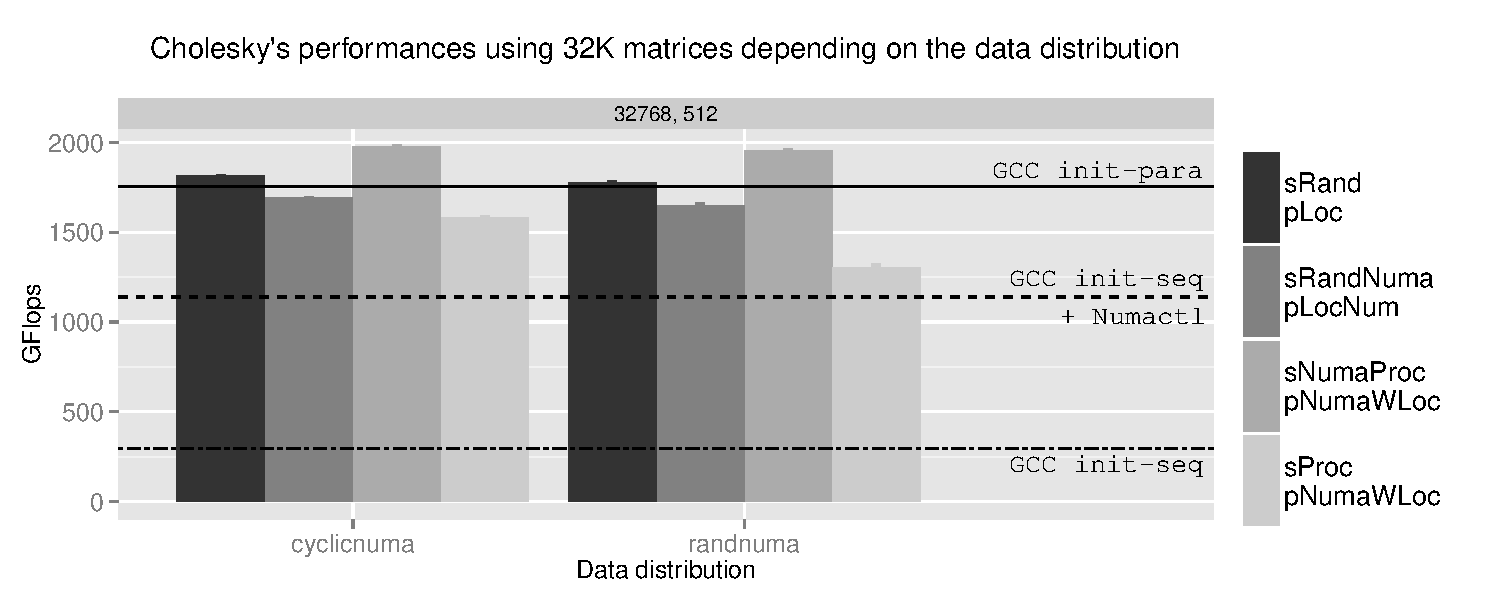
\includegraphics[scale=0.5]{figures/graph_distrib.pdf}
  \caption{Evaluating data distributions for multiple strategies (WSselect + WSpush)}
\label{fig:eval-distrib}
\end{figure}

Using \verb/numactl/ provides an important performance gain compared to the sequential initialization.
However using a parallel initialization, either controlled (\verb/cyclicnuma/, \verb/randnuma/) or
not (GCC init-para), is necessary to significantly improve the performances, regardless of the strategies used.

The \verb/cyclicnuma/ distribution is the one that works best regardless of
the strategies, and we will use it as the default strategy for the next experiments.



\subsection{Impact of the stealing restriction}

Given a data distribution, previous works~\cite{Olivier:2012:CMW:2388996.2389085}
have shown that restricting the task execution to the node where the data are
written leads to better data locality which may improve the application performance.
%Note explicative :
% Pour i dans 0-N le kernel dpot agit sur chaque bloc de la diagonale
% Au rang i,
% - trsm agit sur la colonne en dessous de la case i,i
% - syrk agit sur toutes les cases de la diagonale à partir de i+1,i+1 jusqu'à n,n
% - gemm agit sur le reste des cases de la triangulaire inférieure non touchées par trsm ou syrk
% Bref : il y a 64 tiles en round robin, ça fait un peu moins de 3 tiles/noeuds, sur 64 tiles
% seulement 36 sont écrites, parmis elles la colonne inférieure 1 est écrite 1 fois,
% la 2 deux fois, etc. Chaque case i,i est écrite i+1 fois, les dépendances
% en écriture sont donc très largement concentrées sur la partie inférieure droite de la matrice !
% Donc le strict c'est nul.
However, this is heavily dependent on the algorithm the application implements. For instance, in the case
of a Cholesky factorization, many tasks write to the diagonal tiles
of the matrix comparatively to other tiles of the matrix. Therefore applying
a steal restriction on these tasks will potentially lead to an important number
of inactive processors.
We evaluated both strict and loose versions of our work-stealing strategies and found
out that preventing processors from stealing from other NUMA nodes can lead to a loss of performance by
around 25\% to more than 75\% with respect to the same setup without the \emph{strict}
restriction.
For the sake of brevity we did not include a figure for this, but the results of these
experiments are included in the logs publicly published.

%\begin{figure}[t]
  %\centering
  %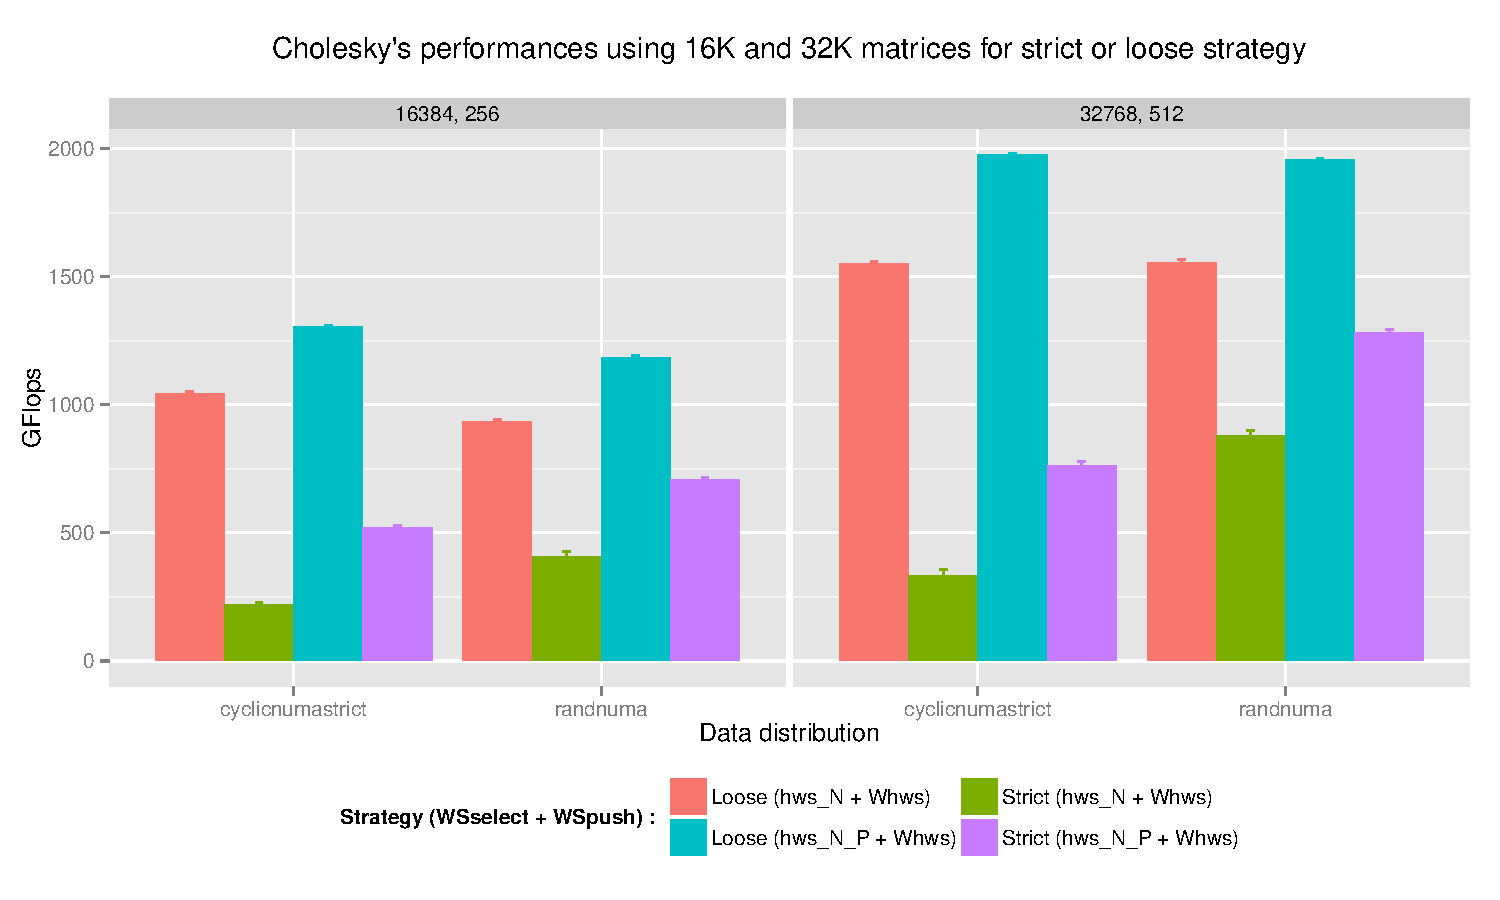
\includegraphics[scale=0.6]{figures/graph_strict.pdf}
%\caption{Evaluating impact of strictness}
%\label{fig:eval-strict}
%\end{figure}


\subsection{Overview of the strategies performances}

We took a given data distribution, \verb/cyclicnuma/, and compared the different strategies, without any steal restriction.
The performance obtained running the Cholesky application 
executed by the libGOMP~\footnote{GCC 5.2.0} runtime system (without modification) is considered as a baseline for these experiments.
Once again, even if the performances we obtained are obviously not the same, the behavior of the different strategies comparatively to each others are similar for the different applications we ran.
Figure \ref{fig:eval-all-strat} shows the results of the experiments for the
Cholesky application on 32K-wide matrices divided into blocks of 512$\times$512 elements (best configuration for this matrix size).
The dashed horizontal line is the GCC performance baseline using parallel initialization.

It is first interesting to note that even very basic \verb/WSselect/
and \verb/WSpush/ strategies, like \verb/sRand/+\verb/pLoc/, obtained decent performances
thanks to the data distribution.
Also, given a selection strategy (e.g. \verb/sRandNuma/), placing
the task on the NUMA node where the written data are allocated (\verb/pNumaW/) behaves better than simply pushing the data to its NUMA node (\verb/pLocNum/).
However, assuming the tasks are being pushed using the \verb/pNumaWLoc/ strategy, focusing the
place selection on only one level of the hierarchy (\verb/sProc/ or \verb/sNuma/)
fails to reach the same level of performance we obtained with naive strategies.
On the contrary, taking into account both levels of the hierarchy (\verb/sProcNuma/,
\verb/sNumaProc/) achieve similar performance that outperforms other strategies.

\begin{figure}[t]
  \centering
  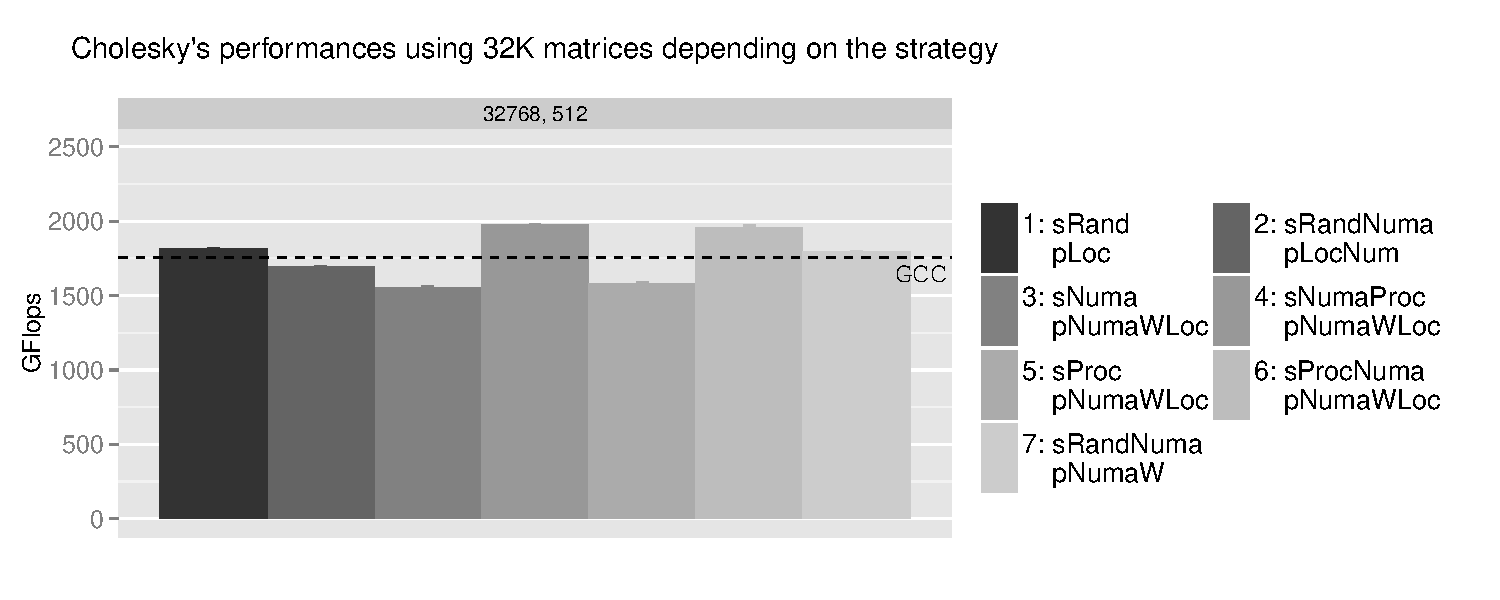
\includegraphics[scale=0.5]{figures/graph_all_strat.pdf}
  \caption{Evaluating all strategies (WSselect + WSpush)}
\label{fig:eval-all-strat}
\end{figure}

\subsection{Strategies performance scaling}

\begin{figure}[t]
  \centering
  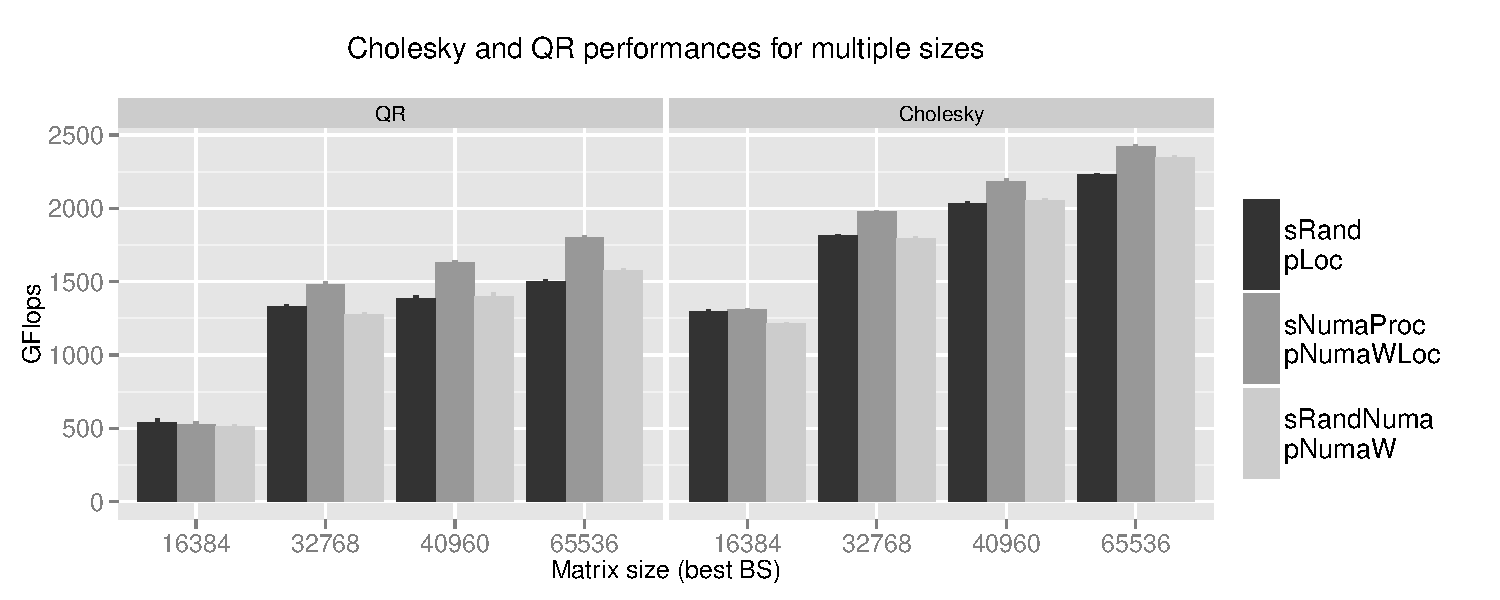
\includegraphics[scale=0.5]{figures/graph_details_strat.pdf}
\caption{Evaluating specific strategies on multiple sizes}
\label{fig:eval-strat-sizes}
\end{figure}

We eventually selected the three strategy combinations that outperformed the GCC baseline to evaluate their scalability depending on the size of the input matrix.
These strategy combinations are :
\begin{itemize}
  \item \verb/sRand/ + \verb/pLoc/, which is a basic strategy that does not take the architecture topology into account ;
  \item \verb/sNumaProc/ + \verb/pNumaWLoc/, which was the best strategy in our previous
    evaluation and is also equivalent to using \verb/sProcNuma/ ;
  \item \verb/sRandNuma/ + \verb/pNumaW/ that performs random selection of node-level places.
\end{itemize}

Figure \ref{fig:eval-strat-sizes} reports their performances using a \verb/cyclicnuma/ distribution without steal restriction.
The figure shows the performances using the best block size for each matrix size (which is, for our setup, 256 for a matrix
size of 16384, and 512 for the others).
As expected, combinations of strategies taking both the architecture hierarchy and data locality into account (\verb/sNumaProc/
+ \verb/pNumaWLoc/) achieve the best performances.
The only exceptions are for small matrix sizes (16384), where there may just be
not enough work to be able to take advantage of this strategy.
We must note that simply distributing the data over the nodes enables the basic
\verb/sRand/ + \verb/pLoc/ combination to achieve satisfying performances.

\section{Related work}
\label{sec:related-work}

Numerous works focus on data locality and/or topology-aware task scheduling strategies for
NUMA architectures.
Clet-Ortega et al.~\cite{DBLP:conf/europar/Clet-OrtegaCP14} studied different ways of decorating the architecture topology with task lists and how it impacts the performance of task-based applications on NUMA systems, promoting private per-threads lists of tasks browsed in a hierarchical way by work-stealing strategies.
We somehow extended this work considering also node-level task lists. We showed considering these lists for pushing ready tasks and selecting work-stealing victims can help improving performance on NUMA systems.
Olivier et al.~\cite{DBLP:journals/ijhpca/OlivierPWSP12} evaluated hierarchical task scheduling with respect to traditional centralized or distributed task schedulers. Creating a thread list, called \emph{shepherd}, per NUMA node allowed their hierarchical scheduler to outperforms other approaches on several task-based applications.
Tahan et al.~\cite{DBLP:journals/corr/Tahan14} also studied the behavior of task-based OpenMP applications on NUMA systems, extending the NANOS runtime system with two NUMA-aware task schedulers called DFWSPT and DFWSRPT, taking into account the notion of task priority when pushing tasks to core-level queues. They also try to minimize the number of \emph{memory hops} when performing load balancing.
While the same kind of studies have been conducted in other contexts~\cite{DBLP:conf/europar/TerbovenSCM12,DBLP:journals/corr/abs-1101-0093}, none of them takes advantage of the OpenMP \verb/depend/ clause, which precisely indicates which data are read and written by a given task. As advertised by the results obtained by our \verb!sNumaProc+pNumaWLoc! combined strategy, this information is worth taking into account when choosing a place to push ready tasks to.

%TODO parler des schedule static.


\section{Conclusion and future work}
Task-based programming environments like OpenMP have become a standard way to program large-scale NUMA systems.
Indeed, they give the programmer ways of expressing massive fine-grain parallelism that can be dynamically mapped to the architecture topology at runtime.
OpenMP recently evolved to deal with tasks dependencies describing the data a task reads as input and writes as output. 

This paper presented several runtime-level strategies to efficiently assign tasks to processors on any NUMA architecture. We presented strategies assigning ready tasks to lists of tasks, called \emph{places}, attached to processors and NUMA nodes. These strategies define the way a task-based runtime system pushes ready tasks to their initial place and the way idle processors browse the architecture topology to select a place to steal from. We considered several initial data distributions and evaluated different combinations of "push" and "select" strategies on a 192 core NUMA system, on linear algebra applications. We achieved the best performance with strategies taking into account both the architecture topology and the initial data placement obtained through OpenMP tasks dependencies.

A short-term future work will be to extend an OpenMP compiler to be able to identify the initialization tasks in a more OpenMP-friendly manner, like extending the \verb!task! construct with a \verb!init! clause. We also intend to experiment with more OpenMP 4 applications.
In a longer term, we intend to move our focus to compile-time techniques able to infer and to attach valuable information on tasks, like an estimation of a task operational intensity, that could guide some of the runtime system's decisions regarding task scheduling and load balancing. We strongly believe a tight cooperation between the compiler and the runtime system is a key step to enhance the performance and scalability of task-based programs on large-scale platforms.

\vspace*{-2ex}
\section*{Acknowledgments}

PIA ELCI - Software environment for computation-intensive applications funded by the French government.

\bibliography{Bib/paper.bib}

\end{document}






